%Para slide em "Wide-Screen" usar:
\documentclass[aspectratio=43]{beamer} 

%Para slide "quadrado" usar:
%\documentclass{beamer} 

\usepackage{tikz}

%Elaborado por Mateus Moro Lumertz

\author{mateuslumertz}
\definecolor{cor1}{RGB}{0,100,166}
\definecolor{cor2}{RGB}{100,195,213}
\definecolor{cor5}{RGB}{150,203,226}
\definecolor{cor3}{RGB}{30,130,186}
\definecolor{cor4}{RGB}{40,185,218}
\definecolor{preto}{RGB}{0,0,0}
\definecolor{branco}{RGB}{255,255,255}
% Configuração das Cores
\setbeamercolor{paleta1}{fg=cor1,bg=white}
\setbeamercolor{paleta2}{fg=cor1,bg=white}
\setbeamercolor{estrutura}{fg=cor1,bg=white}
\setbeamercolor{titulo_rodape}{fg=black,bg=white}
\setbeamercolor{data_rodape}{fg=gray,bg=white}
\setbeamercolor{frametitle}{fg=branco,bg=cor1}

% Modelo do rodapé
\defbeamertemplate*{footline}{mytheme}{%
  \leavevmode%
  \hbox{\begin{beamercolorbox}[wd=.5\paperwidth,ht=2.5ex,dp=1.125ex,leftskip=.3cm,rightskip=.3cm]{titulo_rodape}%
    \makebox[2em][l]{{\usebeamerfont{titulo_rodape}\textcolor{cor1}{\insertframenumber}}}%
    {\usebeamercolor{titulo_rodape}\insertshorttitle}
  \end{beamercolorbox}%
  \begin{beamercolorbox}[wd=.2\paperwidth,ht=2.5ex,dp=1.125ex,leftskip=.3cm,rightskip=.3cm]{data_rodape}%
    \usebeamerfont{data_rodape}\insertshortdate%
  \end{beamercolorbox}%
  \begin{beamercolorbox}[wd=.3\paperwidth,ht=2.5ex,dp=1.125ex,leftskip=.3cm,rightskip=.3cm,right]{titulo_rodape}%
    
\includegraphics[width=.2\paperwidth,height=7ex,keepaspectratio]{imagens/logo.png}\hspace*{2em}%
  \end{beamercolorbox}}%
  \vskip0pt%
}

% Slide de Título
\defbeamertemplate*{title page}{mytheme}[1][]
{%
  \begin{tikzpicture}[remember picture,overlay]
    \filldraw[cor1]
    (current page.north west) --
    ([yshift=-12cm]current page.north west) --
    ([xshift=-4cm,yshift=-12cm]current page.north east) {[rounded corners=15pt]--
    ([xshift=-4cm,yshift=3cm]current page.south east)} --
    ([yshift=3cm]current page.south west) --
    (current page.south west) --
    (current page.south east) --
    (current page.north east) -- cycle
    ;
  \filldraw[branco]
    (current page.north west) --
    ([yshift=-2.15cm]current page.north west) --
    ([xshift=-3cm,yshift=-2.15cm]current page.north east) {[rounded corners=15pt]--
    ([xshift=-3cm,yshift=3cm]current page.south east)} --
    ([yshift=3cm]current page.south west) --
    (current page.south west) --
    (current page.south east) --
    (current page.north east) -- cycle
    ;
    \filldraw[cor2]
    ([xshift=-0.25cm,yshift=3cm]current page.south east)--
    ([xshift=-2.75cm,yshift=3cm]current page.south east)--
    ([xshift=-2.75cm,yshift=3.85cm]current page.south east)--
    ([xshift=-0.25cm,yshift=3.85cm]current page.south east)-- cycle
    ;
    \filldraw[cor3]
    ([xshift=-0.25cm,yshift=4cm]current page.south east)--
    ([xshift=-2.75cm,yshift=4cm]current page.south east)--
    ([xshift=-2.75cm,yshift=4.85cm]current page.south east)--
    ([xshift=-0.25cm,yshift=4.85cm]current page.south east)-- cycle
    ;
    \filldraw[cor4]
    ([xshift=-0.25cm,yshift=5cm]current page.south east)--
    ([xshift=-2.75cm,yshift=5cm]current page.south east)--
    ([xshift=-2.75cm,yshift=5.85cm]current page.south east)--
    ([xshift=-0.25cm,yshift=5.85cm]current page.south east)-- cycle
    ;
    \filldraw[cor5]
    ([xshift=-0.25cm,yshift=6cm]current page.south east)--
    ([xshift=-2.75cm,yshift=6cm]current page.south east)--
    ([xshift=-2.75cm,yshift=6.85cm]current page.south east)--
    ([xshift=-0.25cm,yshift=6.85cm]current page.south east)-- cycle
    ;
  \node[text=branco,anchor=south west,font=\sffamily\LARGE,text width=.68\paperwidth] 
  at ([xshift=10pt,yshift=-0.5cm]current page.west)
  (title)
  {\raggedright\inserttitle};  
  
  \node[text=cor1,anchor=south west,font=\sffamily\small,text width=.75\paperwidth] 
  at ([xshift=10pt,yshift=3.6cm]current page.west)
  (title)
  {\raggedright Université Côte d'Azur};  
  
  \node[anchor=east]
  at ([xshift=-0.15cm,yshift=-1cm]current page.north east)
  {
\includegraphics[width=2.5cm]{imagens/logo.png}};
  
  \node[text=preto,font=\large\sffamily,anchor=south west]
  at ([xshift=30pt,yshift=0.5cm]current page.south west)
  (date)
  {\insertdate};
  \node[text=preto,font=\large\sffamily,anchor=south west]
  at ([yshift=5pt]date.north west)
  (author)
  {\insertauthor};
  \end{tikzpicture}%
}

% remove navigation symbols
\setbeamertemplate{navigation symbols}{}

% definition of the itemize templates
\setbeamertemplate{itemize item}[circle]
\setbeamercolor{itemize item}{fg=cor3,bg=white}
\setbeamercolor{itemize subitem}{fg=cor4,bg=white}
\setbeamercolor{itemize subsubitem}{fg=cor2,bg=white}

%%%%%%%%%%%%%%%%%%%%%%%%%%%%%%%%%%%%%%%%%%%%%%%%%%%%%%%%%%%%%%%%%%%%
%%%%%%%%%%%%%%%%%%%%%%%%%%%%%%%%%%%%%%%%%%%%%%%%%%%%%%%%%%%%%%%%%%%%
%%%%%%%%%%%%%%%%%%%%%%%%%%%%%%%%%%%%%%%%%%%%%%%%%%%%%%%%%%%%%%%%%%%%
%%%%%%%%%%%%%%%%%%%%%%%%%%%%%%%%%%%%%%%%%%%%%%%%%%%%%%%%%%%%%%%%%%%%
%%%%%%%%%%%%%%%%%%%%%%%%%%%%%%%%%%%%%%%%%%%%%%%%%%%%%%%%%%%%%%%%%%%%

\title[NHS and GDPR]{Analysis of the National Health Service's GDPR status}
\author{Charles Canavaggio, Enrico Bachiorrini, Quentin Le Roux}
\date{\today}

\begin{document}

\begin{frame}[plain]
\maketitle
\end{frame}

% %Slide 
% \begin{frame}
%     \frametitle{Introduction}
%     \framesubtitle{subtitle}
%     \begin{itemize}
%         \item 
%     \end{itemize}
%     
\includegraphics[width=0.4\linewidth]{imagens/logo.png}
% \end{frame}

\begin{frame}
    \frametitle{The NHS and GDPR}
    \framesubtitle{Does GDPR apply to NHS}
    \begin{itemize}
        \item Brexit: the UK has left the EU on December 31st, 2020\newline
        \item The UK, without a data adequacy agreement is considered a 'third country' under GDPR\newline
        \item British data officers will have to take mitigating actions\newline
        \item The NHS is affected
    \end{itemize}
\end{frame}

\begin{frame}
    \frametitle{Website Registration}
    \framesubtitle{Location of the website}
    The NHS' website is registered in the UK.\newline\newline
    	\begin{quote}
    	\textit{\% IANA WHOIS server}\newline
        refer:        whois.nic.uk\newline
        domain:       UK\newline
        organisation: Nominet UK\newline
        address:      Minerva House\newline
        address:      Edmund Halley Road\newline
        address:      Oxford Science Park\newline
        address:      Oxford  OX4 4DQ\newline
        address:      United Kingdom
        \end{quote}
\end{frame}

\begin{frame}
    \frametitle{The NHS and potential EU-based users}
    \framesubtitle{Does the NHS provide services to EU-based users}
    \begin{itemize}
        \item The UK has large population exchanges with Europe\newline
        \item  GDPR Art. 3 on "Territorial Scope": GDPR applies to data processing within the EU regardless of the data subjects' origin\newline
        \item Many British citizens live, work, visit the EU and are entitled to services from the NHS\newline
    \end{itemize}
    $\Rightarrow$ The NHS has to adhere to GDPR when dealing with users located in the EU
\end{frame}

\begin{frame}
    \frametitle{NHS' cookie banner}
    \framesubtitle{Does the NHS show a cookie banner?}
    The NHS' website displays a prominent cookie banner at the top of its front page.
    \newline
    \newline
    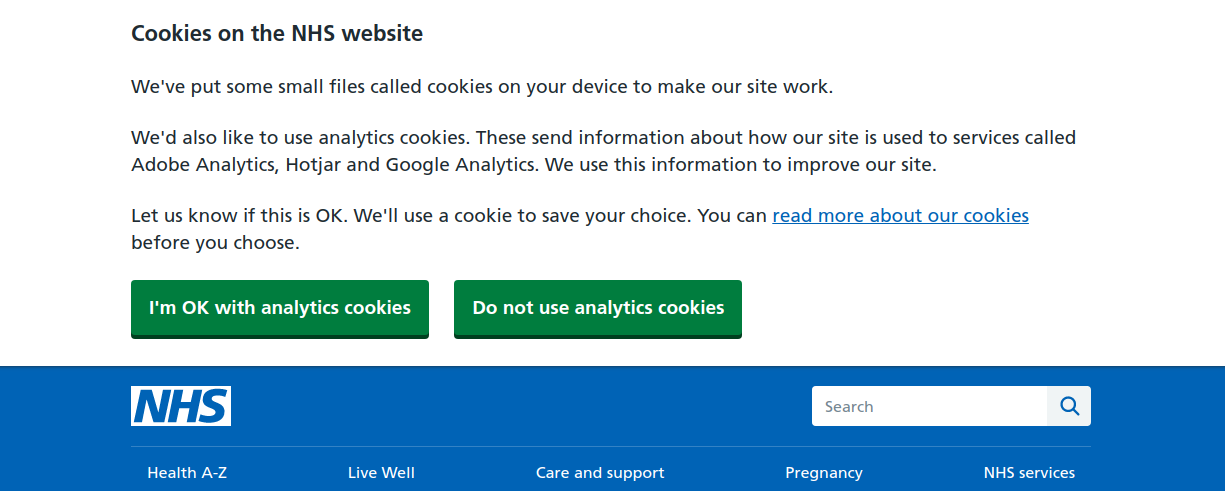
\includegraphics[width=0.9\linewidth]{imagens/nhs_cookie_bar.png}
\end{frame}

%Slide 
\begin{frame}
    \frametitle{NHS' cookie banner}
    \framesubtitle{Analysis of consent on the website in the context of GDPR - 1}
    \begin{itemize}
        \item Prior
        \begin{itemize}
            \item Prior to storing an identifier
            \item Prior to sending an identifier
        \end{itemize}
        \item Free
        \begin{itemize}
            \item No merging into a contract
            \item No tracking walls
        \end{itemize}
        \item Specific
        \begin{itemize}
            \item Separate consent per purpose
        \end{itemize}
        \item Informed
        \begin{itemize}
            \item Accessibility of information page
            \item Necessary information on BTT
            \item Information on consent banner configuration
            \item Information on the data controller
            \item Information on rights
        \end{itemize}
    \end{itemize}
\end{frame}

\begin{frame}
    \frametitle{NHS' cookie banner}
    \framesubtitle{Analysis of consent on the website in the context of GDPR - 2}
    \begin{itemize}
        \item Unambiguous
        \begin{itemize}
            \item Affirmative action design
            \item Configurable banner
            \item Balanced choice
            \item Post-consent registration
            \item Correct consent registration
        \end{itemize}
        \item Readable and accessible
        \begin{itemize}
            \item Distinguishable
            \item Intelligible
            \item Accessible
            \item Clear and plain language
            \item No consent wall
        \end{itemize}
        \item Revocable
        \begin{itemize}
            \item Possible to change in the future
            \item Delete "consent cookie" and communicate to third parties
        \end{itemize}
    \end{itemize}
\end{frame}


\begin{frame}
    \frametitle{NHS' privacy and cookie policies}
    \framesubtitle{Does the website provide a privacy or cookie policy?}
    \begin{itemize}
        \item The website provides both a cookie policy and privacy policy\newline
        \item GDPR Art.4's personal data definition and Art.3 territoriality clause imply data collected by the NHS is considered as personal in some specific cases (e.g. British citizens living in the EU)\newline
        \item Legal basis of action: The privacy policy clearly states the legal bases of their use of personal data (Data Protection Act of 2018, GDPR, and a total of 52 other directives cover the whole legal basis of the NHS' data collection and processing)
    \end{itemize}
\end{frame}

%Slide 
\begin{frame}
    \frametitle{NHS' privacy and cookie policies}
    \framesubtitle{Analyse the policies of the website}
    Cookie Policy's stated data usage purposes:
    \begin{itemize}
        \item Make the website work
        \item Remember pop-ups
        \item Analytics cookies
        \item Ads of health campaigns\newline
    \end{itemize}
    Privacy Policy's context:
    \begin{itemize}
        \item Data controller: Health and Social Care Information Centre (i.e. NHS Digital)
        \item Data processors: the NHS itself is the main data processor, for which others may act on behalf (e.g. NHS Improvement, NHS' Data Processing Services, Health Data Research UK)
        \item Third-Party data processors: 5 are referenced (see next slide)
    \end{itemize}
\end{frame}

\begin{frame}
    \frametitle{Third-Parties}
    \framesubtitle{Analysis of the third-parties on the site}
    5 third-parties involved in the management of website cookies: New Relic, Adobe Analytics, Google Analytics, Hotjar, Qualtrics. The last four provide a suite of tools to the NHS that involve processing of personal data.\newline
    \begin{itemize}
        \item Third-parties are specifically mentioned in the cookie banner
        \item Third parties are described exhaustively in the cookie and privacy policies
        \item The NHS links to the privacy policy of each of the 5 third-parties\newline
    \end{itemize}
    Some third-parties that do not involve personal data are also mentioned (such as CloudFare)
\end{frame}

\begin{frame}
    \frametitle{Conclusions}
    \framesubtitle{Overall impressions}
    \begin{itemize}
    \item The NHS likely complies with the current GDPR rules\newline
    \item The new status of the UK as a third country since January 1st, 2021, and the lack of a data adequacy agreement with the EU implies a certain amount of uncertainty
    \end{itemize}
\end{frame}


\end{document}